\chapter{Evaluation}

% \textit{Note: If you did an evaluation / case study, describe it here.}

\section{Design}

% \textit{Note: Describe the design / methodology of the evaluation and why you did it like that. E.g. what kind of evaluation have you done (e.g. questionnaire, personal interviews, simulation, quantitative analysis of metrics, what kind of participants, what kind of questions, what was the procedure?}

The evaluation process was done to assess both the functional and non-functional requirements of the system.
This evaluation is done by processing the data collected from the users by the application.
The python library numpy and pandas are used to process the data.
Numpy is used to perform mathematical operations on the data and pandas is used to visualize the data.
If the system was able to collect and store data accurately, then the system is considered to be functioning correctly.
Whether the data being saved is accurate or not should be clear through the evaluation process.

\section{Objectives}

% \textit{Note: Derive concrete objectives / hypotheses for this evaluation from the general ones in the introduction.}

The data can be compared to the expected data to see if the system is functioning correctly.
An example of this would be to compare the average typing speed from the collected data and average typing speed data from other sources.
On average, the typing speed of a person on mobile devices is 36.2 \ac{WPM} with 2.3\% uncorrected errors \cite{Palin2019}.
This translate to 331.49 ms average duration between keystrokes, if we consider that on average, there are 5 characters per word.

Typing speed also varies depending ont he age of the user.
Age group 10-19 has the fastest typing speed with 39.6 \ac{WPM} and age group 50-59 has the slowest typing speed with 26.3 \ac{WPM} \cite{Palin2019}.
This translates to average speed between keystrokes of 303.03 ms for 39.6 \ac{WPM} and 456.65 ms for 26.3 \ac{WPM}.
This is the expected average duration between keystrokes for the data that has been collected by the application.

\section{Results}

% \textit{Note: Summarize the most interesting results of your evaluation (without interpretation). Additional results can be put into the appendix.}

\begin{table}[h]
    \centering
    \begin{tabular}{ccccc}
    \toprule
    \textbf{Age Group} & {Conversations} & Message Count & Message Length (Mean) \\
    \midrule
    0-24     & 7 & 26 & 19.77 \\
    25-39    & 9 & 39 & 53.59\\
    40-59    & 18 & 103 & 48.56\\
    60+      & 6 & 30 & 32.17 \\
    \bottomrule
    \end{tabular}
    \caption{Amount of unique conversations of each age groups.}
    \label{tab:unique_conversations}
\end{table}

\begin{figure}[h!]
    \centering
    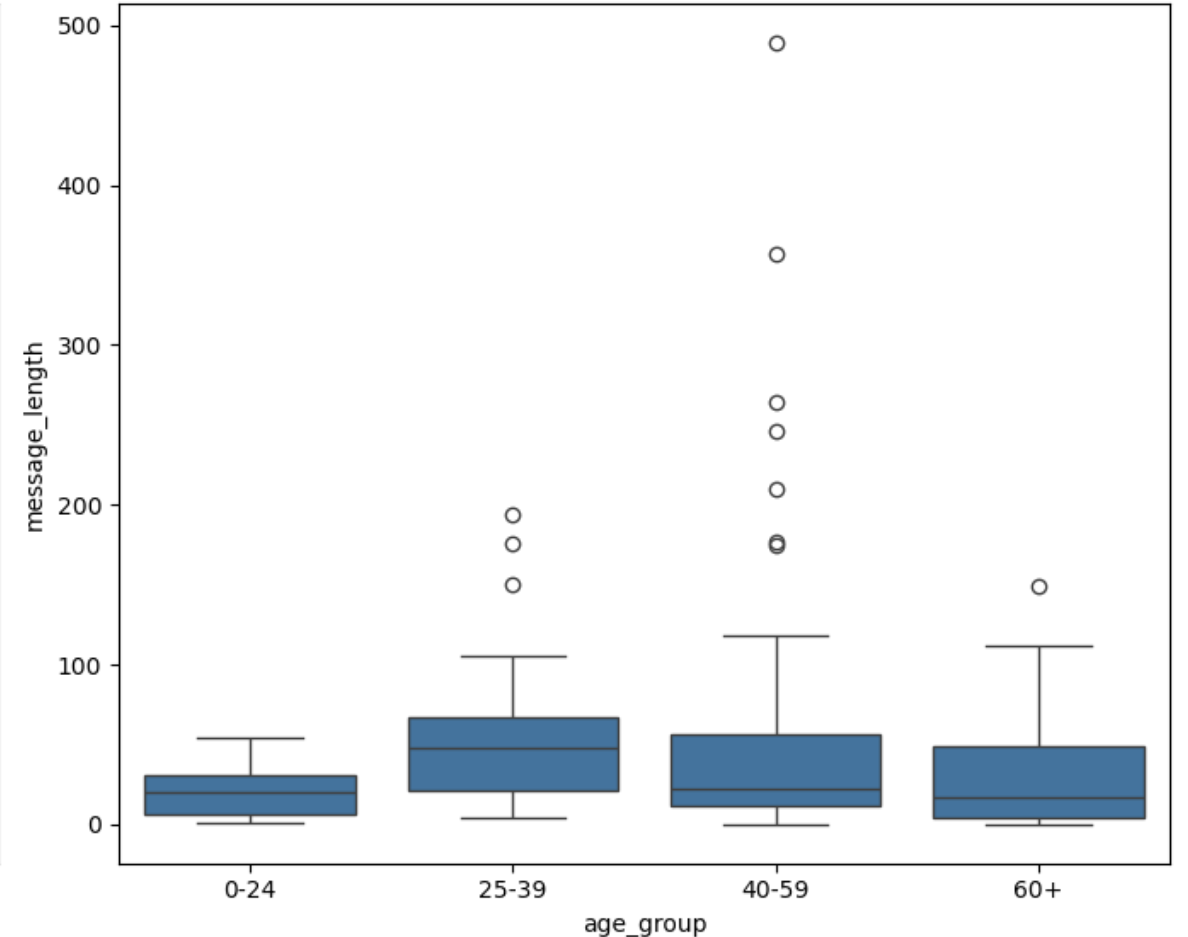
\includegraphics[width=13cm]{message_length.png}
    \caption{Box plot of message length of each age group.}
    \label{box_plot_message_length}
\end{figure}


Table \ref{tab:unique_conversations} shows the number of unique conversations, number of messages sent and the average length of the message sent.
In total, the application managed to gather data from 40 unique conversations.
Age group 40-59 has the most unique conversations with 18 conversations and most message sent with 103 messages.
Meanwhile age group 60+ has the least unique conversations with 6 conversations.
The least amount of messages sent is by age group 0-24 with 26 messages.

Regarding message length average, age group 25-39 has the longest message length average with 53.59 characters.
Age group 40-59 has the second longest message length average with 48.56 characters.
Age group 0-24 has the shortest message length average with 19.77 characters.

\begin{table}[h]
    \centering
    \begin{tabular}{ccccc}
    \toprule
    \textbf{Age Group} & Backspace Percentage (Mean) \\
    \midrule
    0-24     & 6.00 \\
    25-39    & 6.63 \\
    40-59    & 15.93 \\
    60+      & 3.29 \\
    \bottomrule
    \end{tabular}
    \caption{Average of backspace percentage of each age groups.}
    \label{tab:backspace_percentage}
\end{table}

Table \ref{tab:backspace_percentage} shows the average backspace percentage of each age group.
Backspace percentage is calculated by dividing the number of backspace keystrokes by the total number of keystrokes.
Age group 40-59 has the highest backspace usage percentage with 15.93\%.
Age group 0-24 has the lowest backspace usage percentage with 6.63\%.


\begin{table}[h]
    \centering
    \begin{tabular}{ccccc}
    \toprule
    \multicolumn{1}{c}{} & \multicolumn{2}{c}{\textbf{Typing Speed}}\\
    \cmidrule(rl){2-3} \cmidrule(rl){4-5}
    \textbf{Age Group} & {Mean (ms)} & {Std. Dev (ms)} \\
    \midrule
    0-24 & 241.54 & 199.47 \\
    25-39 & 272.87 & 128.61  \\
    40-59 & 386.99 & 188.92 \\
    60+ & 285.72 & 137.01 \\
    \bottomrule
    \end{tabular}
    \caption{Typing speed of users in different age groups.}
    \label{tab:typing_behavior}
\end{table}

\begin{figure}[h!]
    \centering
    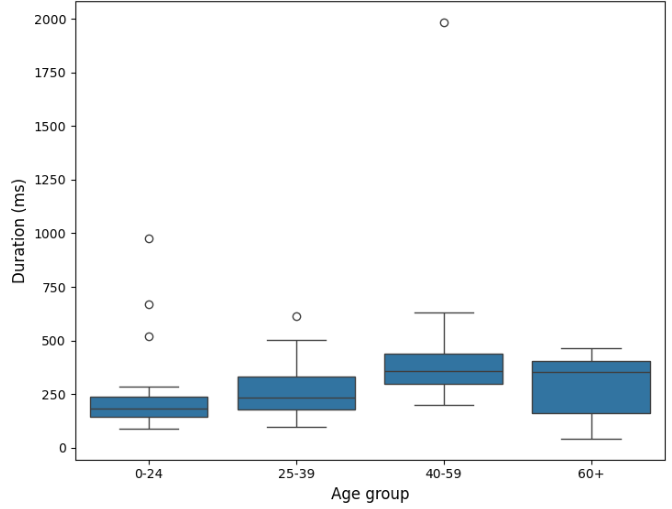
\includegraphics[width=13cm]{typing_speed.png}
    \caption{Box plot of typing speed of each age group.}
    \label{box_plot_typing_speed}
\end{figure}

During the processing of the data, keysrokes duration that took longer than five seconds are truncated.
This is done to remove data that is most likely caused by trivial factors, such as the user being away from keyboard.
Table \ref{tab:typing_behavior_one} shows the average and standard deviation of duration between each keystrokes after the data is truncated.

Age group 0-24 shows the fastest typing speed with an average duration of 241,54 ms between each keystrokes.
This age group also shows the highest versatility in typing speed with a standard deviation of 199,47 ms.

Age group 25-39 shows a slower typing speed than the previous age group.
This is, however, the second fastest typing speed with an average duration of 272,87 ms between each keystrokes.
This age group is also the least variable in typing speed with a standard deviation of 128,61 ms.

Age group 40-59 shows the slowest typing speed with an average duration of 386,99 ms betwen each keystrokes.
This age group also shows high versatility in typing speed with a standard deviation of 188,92 ms.

Average typing speed of age group 60+ increases compared to age group 40-59.
This age group has the second slowest typing speed with an average duration of 285,72 ms between each keystrokes.

\begin{table}[h]
    \centering
    \begin{tabular}{ccccc}
    \toprule
    \multicolumn{1}{c}{} & \multicolumn{2}{c}{\textbf{Typing Speed}}\\
    \cmidrule(rl){2-3} \cmidrule(rl){4-5}
    \textbf{Age Group} & {Mean (ms)} & {Std. Dev (ms)} \\
    \midrule
    0-24 & 226.94 & 193.75 \\
    25-39 & 253.15 & 123.82  \\
    40-59 & 357.05 & 189.69 \\
    60+ & 279.32 & 132.83 \\
    \bottomrule
    \end{tabular}
    \caption{Typing speed of users in different age groups with truncation.}
    \label{tab:typing_behavior_one}
\end{table}

\begin{figure}[h!]
    \centering
    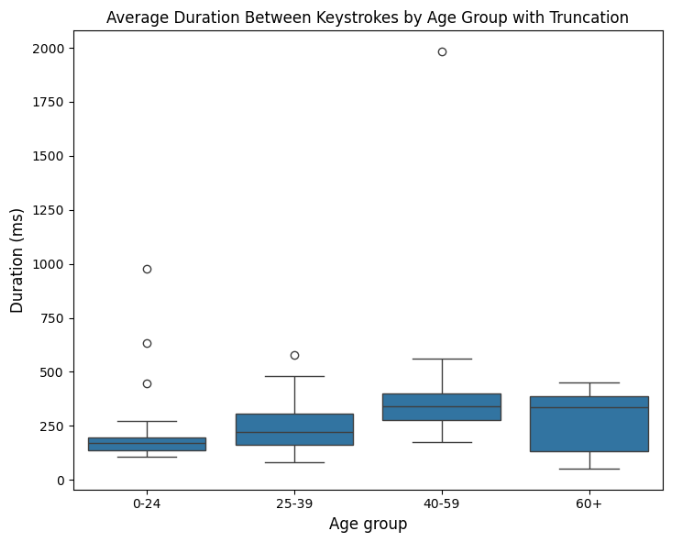
\includegraphics[width=13cm]{typing_speed_two_seconds.png}
    \caption{Box plot of typing speed of each age group with truncation.}
    \label{box_plot_typing_speed_two_seconds}
\end{figure}

Next, the data is truncated further by removing the one-percenth quantile (\textless1\% and \textgreater99\%) of duration between keystrokes.
This is done to remove outliers from the data.
Table \ref{tab:typing_behavior_one} shows the average and standard deviation of duration between each keystrokes after data processing is done.

Age group 0-24 shows the fastest typing speed with an average duration of 226,94 ms between each keystrokes.
Similar to the previous evaluation, this age group also shows the highest versatility in typing speed with a standard deviation of 193,75 ms.

Age group 25-39 is slightly slower, with an average duration of 253,15 ms between each keystrokes.
This is, however, still the second fastest typing speed.
This group also has the least variable typing speed with a standard deviation of 123,82 ms.

Age group 40-59 has the slowest typing speed with an average duration of 357,05 ms betwen each keystrokes.
Versatility in typing speed of this group is high with a standard deviation of 189,69 ms.

For age group 60+ the average typing speed is slightly faster than age group 40-59.
This age group has the second slowest typing speed with an average duration of 279,32 ms between each keystrokes.
Versatility in typing speed of this group is low with a standard deviation of 132,83 ms.

\begin{table}[h]
    \centering
    \begin{tabular}{ccccc}
    \toprule
    \multicolumn{1}{c}{} & \multicolumn{2}{c}{\textbf{Typing Speed}}\\
    \cmidrule(rl){2-3} \cmidrule(rl){4-5}
    \textbf{Age Group} & {Mean (ms)} & {Std. Dev (ms)} \\
    \midrule
    0-24 & 195.69 & 117.00 \\
    25-39 & 253.84 & 121.98  \\
    40-59 & 344.07 & 82.60  \\
    60+ & 274.03 & 132.96 \\
    \bottomrule
    \end{tabular}
    \caption{Typing speed of users in different age groups with \ac{IQR} method.}
    \label{tab:typing_behavior_iqr}
\end{table}


\begin{figure}[h!]
    \centering
    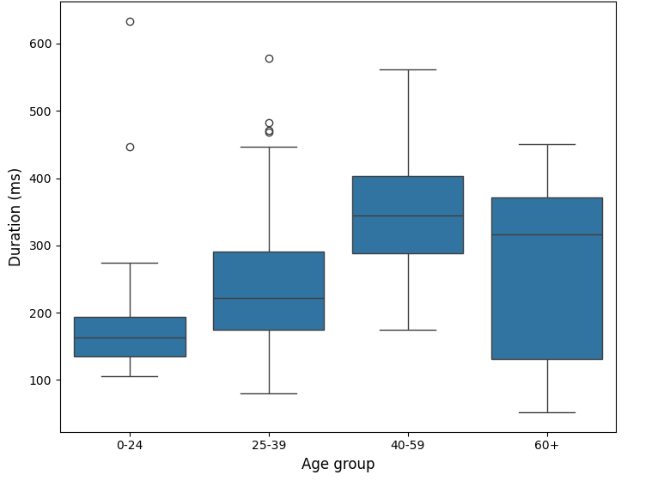
\includegraphics[width=13cm]{iqr.png}
    \caption{Box plot of typing speed of each age group with iqr methods.}
    \label{box_plot_typing_speed_iqr}
\end{figure}

In this evaluation, the data is processed by removing the \ac{IQR} of duration between keystrokes after removing keystrokes that took longer than five seconds.
The ranking of the age groups in terms of average typing speed remains the same with the previous evaluation methods.
However, the ranking of the age groups in terms of versatility in typing speed changes.

Age group 0-24 that was previously the most variable in typing speed is now the second least variable with standard deviation of 117 ms.
Age group 25-39 that was previously the least variable in typing speed is now the second most variable with standard deviation of 121,98 ms.
Age group 40-59 that was previously the second most variable in typing speed is now the least variable with standard deviation of 82,60 ms.
Lastly, age group 60+ that was previously the second least variable in typing speed is now the most variable with standard deviation of 132,96 ms. 

\section{Findings}

% \textit{Note: Interpret the results and conclude interesting findings}
Backspace percentage average increases the older the age group is, except for age group 60+.
A big jump in backspace percentage average is seen between age group 25-39 and 40-59 from 6.63\% to 15.93\%.
Afterwards, the backspace percentage average decreases to 3.29\% for age group 60+.

The data shows that the older the age group, the slower the typing speed.
This is consistent with the general knowledge that the older a person is, the slower their reaction time is.
There is however an exception with age group 60+.
This group has a faster typing speed than age group 40-59 in all of the evaluations.
The fact that this group has the least amount of unique conversations might contribute to this result.

On the first two evaluations, i.e. evaluations without the \ac{IQR} method, if the data for age group 25-39 is left out, there is a trend where the older the age group, the less variable the typing speed is.
Age group 25-39 is, however, an exception to this pattern, as it is the least variable group.
The fact that there are only 9 unique conversations from age gorup 25-39 might contribute to this result.
The standard deviation from the evaluation with the \ac{IQR} method shows no noticeable pattern.

\section{Limitations}

% \textit{Note: Describe limitations and threats to validity of your evaluation, e.g. reliability, generalizability, selection bias, researcher bias}
One of the limitations of the application that becomes apparent during the evaluation is the incapability of knowing whether the conversation is done by typing on the screen or with a physical keyboard.
Typing on a physical keyboard is generally faster than typing on a screen \cite{Varcholik2012}.
This is a limitation of the current version of the application.
Updating the application to also collect data of the media used while using the application should be considered in the future.
This will make sure that the data is more accurate and can be used to make more accurate conclusions.

Another limitation is the fact that the data is gathered from a specific group of people and the small sample size.
This specific group of people might not be representative of the general population, thus impacting the generalizability of the result.
The small sample size also makes the result less reliable.
To improve the reliability of the result, the application should be used by a larger group of people.